\documentclass[11pt,twoside,a4paper]{ctexart}

\usepackage{amsmath}
\usepackage{amssymb}
\usepackage{graphicx}
\usepackage{algorithm}
\usepackage{algorithmicx}
\usepackage{algpseudocode}
\usepackage{hyperref}
\DeclareMathOperator*{\minimize}{minimize}
\floatname{algorithm}{算法}

\begin{document}
\section{元学习简介}
虽然机器学习系统在许多任务上都超过了人类,不过达到同样表现所需的数据量却远远超过人类的,尽管这样的比较并不完全公平,因为人类是带着大量编码在大脑和DNA中的先验知识进入任务的。
人类快速学习的能力可以解释为贝叶斯推断,因此要开发学习读率像人类一样快算法的关键是使算法更加贝叶斯。但实践中,开发使用深度神经网络并使计算可行的贝叶斯机器学习算法十分困难。
最近元学习开始显露出从小样本中快速学习的潜力,它并不尝试模拟贝叶斯推断,而是直使用一个任务集来优化快速学习算法。比如假定有一个任务的分布,每个任务都是一个分类问题,
从这个分布抽取一个任务的训练集和测试集,将训练集输入到算法中,要求算法产生一个在测试集上表现优异的代理。因为每个任务表示一个学习问题,能在一个任务上表现很好就表示学得很快。

少样本元学习的目标是训练一个使用少量数据点和训练迭代就能快速将自己调整到新任务的模型。为此,在元学习阶段用一些任务训练一个模型或学习器,使其仅用少量的样本或尝试就能调整到新任务。
实际上,元学习问题将整个任务集看成是训练样本。考虑一个记为$f$的模型将观测$\mathbf x$映射到输出$\mathbf a$。在元学习期间,训练模型使它能调整到大量的任务,每个任务
$\mathcal T=\left\{\mathcal L(\mathbf x_1, \mathbf a_1, \ldots, \mathbf x_H, \mathbf a_H, ), q(\mathbf x_1), q(\mathbf x_{t+1}\mid\mathbf x_t, \mathbf a_t), H\right\}$
由一个损失函数$\mathcal L$、一个初始观测上的分布$q(\mathbf x_1)$、一个转移分布$q(\mathbf x_{t+1}\mid \mathbf x_t,\mathbf a_t)$和一个片段长度$H$组成。
在独立同分布的监督学习问题中,长度$H=1$。通过在每个时间$t$选择一个输出$\mathbf a_t$模型可以生成长度为$H$的样本。
损失$\mathcal L(\mathbf x_1, \mathbf a_1, \ldots, \mathbf x_H, \mathbf a_H, ) \to \mathbb R$可以误分类损失或马尔可夫代价函数的形式,为模型提供特定任务的反馈。

研究者们已经提出了多种元学习的算法,每种方法都各有优劣:
\begin{itemize}
	\item 在一种方法中,学习算法编码在一个循环神经网络的权值中,但在测试时并不执行梯度下降;
	\item 第二种方法学习初始化网络,然后在测试时用新任务调优。一个典型的例子是使用大数据集预训练并用小数据集调优,但这种典型的预训练方法并不能保证学习到一个适于调优的初始化,
	因此需要专门的技巧。
\end{itemize}

近来Finn等人提出了MAML算法,在调优过程中通过微分,直接对于网络初始化进行优化。在这个方法中,学习者回落到一个基于敏感梯度的学习算法,即使收到样本外的数据;
这是一个模型无关的方法,即兼容于任何用梯度下降训练的方法,并适用于大量不同的学习问题。但另一方面,因为MAML需要通过优化过程微分,并不匹配需要在测试时执行大量梯度步骤的问题。
作者也提出了一个称为一阶MAML(FOMAML)的变体,通过忽略二次导数项来避免了这个问题,同时也发现FOMAML在Mini-ImageNet数据集上的表现几乎和MAML一样好。

\section{MAML}
MAML中,训练模型参数使得少量梯度步骤就能使模型在新任务上产生很好结果的过程,从特征学习的角度可以看成是构建一个广泛适用于许多任务的内部表征。若内部表征适用于许多任务,则仅略微调优参数
(比如主要地调整一个前向模型中的顶层权值),就能产生很好的结果。实际上,这个方法优化来获得容易且快速调优的模型,使得对快速学习的调整发生在正确的空间内。从动态系统的角度这个学习
过程可以看成是:最大化新任务损失函数关于参数的敏感性,当敏感性很高时,参数很小的局部变化就能取得任务损失上很大的改善。

考虑一个希望模型能够调整到的任务分布$p(\mathcal T)$,在$K$样本学习设定中,我们训练模型仅使用来自$q_i$的$K$个样本和来自损失$\mathcal L_{\mathcal T_i}$的反馈来学习
从$p(\mathcal T)$抽取的新任务$\mathcal T_i$。在元学习期间,会从$p(\mathcal T)$抽取一个任务$\mathcal T_i$,然后用$K$个样本和损失$\mathcal L_{\mathcal T_i}$训练模型,
然后在来自$\mathcal T_i$的新样本上测试模型。然后考虑测试错误对应于参数如何变化来模型$f$。实际上,所抽取任务$\mathcal T_i$上的测试错误充当元学习过程的训练误差。在元学习结束时,
从$p(\mathcal T)$抽取新任务,在学习过$K$个样本后,来衡量模型的性能。用于元学习的任务在元学习期间通常会被留出。

MAML能够通过元学习将模型以一种将其为快速调整准备的方式学习任意标准模型的参数。这种方法背后的直觉是一些内部表达比其他的更加可迁移。比如一个神经网络可能学到广泛适用于$p(\mathcal T)$
中所有任务而非单个独立任务的内部特征。采用一种明确的方法来促使这种通用目标的表征发生:既然模型使用基于梯度的学习规则来调优,则致力于以这种基于梯度学习规则能在抽取自$p(\mathcal T)$
新任务获得快速进步而不过拟合的方式学习一个模型。实际上会致力于找到对任务中的变化十分敏感的模型参数,这样当在任意$p(\mathcal T)$中任务的损失函数的梯度方向发生改变时,参数中很小的变化
就会在这个损失上产生很大的改善(见\hyperref[fig1]{图(\ref{fig1})})。模型的形式只依赖于两个假设,一个是模型由某个参数向量$\theta$参数化,另一个是损失函数在$\theta$上足够光滑从而
可以使用基于梯度的学习技术。

\begin{figure}[htbp]
	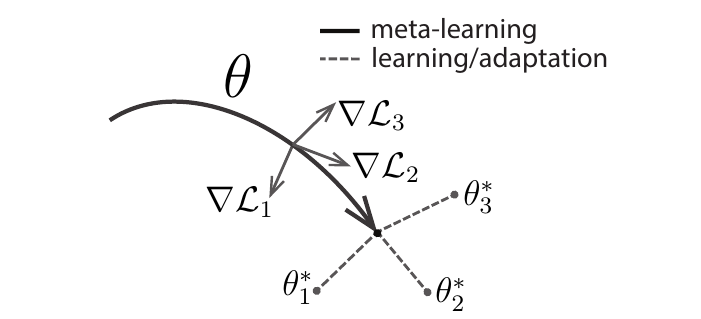
\includegraphics[height=125pt]{fig1}
	\caption{MAML优化来获得一个能够快速调整到新任务的表达$\theta$。}
	\label{fig1}
\end{figure}

形式化而言,考虑一个用参数为$\theta$的参数化函数$f_\theta$表示的模型,当调整到新任务$\mathcal T_i$时,模型的参数$\theta$变为$\theta_i'$。在MAML中,更新的参数向量$\theta_i'$使用
任务$\mathcal T_i$上一个或多个梯度梯度下降的更新来计算。为简化标记,这里仅描述一次梯度更新,但扩展为多个梯度更新也十分直接。因此,
\[ \theta_i' = \theta - \alpha\nabla_\theta\mathcal L_{\mathcal T_i}\left(f_\theta\right) \]
步长参数$\alpha$可以是固定的超参,也可以通过元学习得到。模型参数通过对$f_{\theta_i'}$关于参数$\theta$在$p(\mathcal T)$抽取的任务间的性能优化而得,因此元目标就是:
\[
\min_\theta \sum_{\mathcal T_i \in p(\mathcal T)} \mathcal L_{\mathcal T_i}\left(f_{\theta_i'}\right)
=\sum_{\mathcal T_i \in p(\mathcal T)} \mathcal L_{\mathcal T_i}\left(f_{\theta - \alpha\nabla_\theta\mathcal L_{\mathcal T_i}\left(f_\theta\right)}\right)
\]
注意,元优化在模型参数$\theta$上执行,而目标则使用更新的模型参数$\theta'$计算。任务间的元优化通过SGD执行,因此模型参数的更新为:
\begin{equation}
	\theta \gets \theta - \beta\nabla_\theta \sum_{\mathcal T_i \sim p(\mathcal T)} \mathcal L_{\mathcal T_i}\left( f_{\theta_i'} \right)
\end{equation}
其中$\beta$为元步长,整个的通用算法,见算法。MAML元梯度更新包含一个通过梯度的梯度,计算上需要一个额外通过$f$的反向传播来计算Hessian向量乘积。

\begin{algorithm}
	\caption{模型无关元学习}
	\label{alg1}
	\begin{algorithmic}[1]
		\Require $p(\mathcal T)$:关于任务的分布
		\Require $\alpha,\beta$:步长超参
		\State 随机初始化参数$\theta$
		\While {not done}
			\State 抽取任务批次$\mathcal T_i \sim p(\mathcal T)$
			\For {all $\mathcal T_i$}
				\State 评估$K$个样本的$\nabla_\theta\mathcal L_{\mathcal T_i}\left( f_\theta \right)$
				\State 用梯度下降计算调整参数$\theta'_i=\theta-\alpha\mathcal{L}_{\mathcal{T}_i}\left( f_\theta \right)$
			\EndFor
		\State 更新$\theta \gets \theta - \beta\nabla_\theta\sum_{\mathcal{T}_i\sim p(\mathcal{T})}\mathcal{L}_{\mathcal{T}_i}\left( f_{\theta_i'}\right)$
		\EndWhile
	\end{algorithmic}
\end{algorithm}

\section{监督回归和分类上的MAML}
不同领域间MAML的不同之处在于损失函数的形式和任务生成数据以及呈现给数据的方式。为形式化前面元学习定义语境中的监督回归和分类问题,因为模型接收单个输入并产生单个输出而非输入和输出序列,
因此可以取视野$H=1$,并删除$\mathbf x_t$的时间步下标。任务$\mathcal T_i$从$q_i$产生$K$个独立同分布的观测$\mathbf x$。对回归任务通常使用MSE:
\begin{equation}
	\mathcal{L}_{\mathcal{T}_i}\left(f_\phi\right) = \sum_{\mathbf{x}_j,\mathbf{y}_j\sim\mathcal{T}_i} \left\Vert f_\phi\left(\mathbf x^{(j)}\right)-\mathbf{y}^{(j)} \right\Vert_2^2
\end{equation}
而对分类任务,常用的损失函数为交叉熵损失:
\begin{equation}
	\mathcal{L}_{\mathcal{T}_i}\left(f_\phi\right) = \sum_{\mathbf{x}_j,\mathbf{y}_j\sim\mathcal{T}_i} \mathbf{y}^{(j)}\log f_\phi\left(\mathbf{x}^{(j)}\right)
	+ \left(1-\mathbf{y}^{j}\right)\log\left(1-f_\phi\left(\mathbf{x}^{(j)}\right)\right)
\end{equation}
基于术语习惯,$K$样本分类从每个类别中使用$K$个输入/输出对,因此$N$路分类有$N\times K$个数据点。\hyperref[alg2]{算法(\ref{alg2})}展示了监督学习中执行MAML的细节。
\begin{algorithm}
	\caption{用于监督学习的MAML}
	\label{alg2}
	\begin{algorithmic}[1]
		\Require $p(\mathcal T)$:关于任务的分布
		\Require $\alpha,\beta$:步长超参
		\State 随机初始化参数$\theta$
		\While {not done}
			\State 抽取任务批次$\mathcal T_i \sim p(\mathcal T)$
			\For {all $\mathcal T_i$}
				\State 从$\mathcal{T}_i$抽取$K$个数据点$\mathcal D=\left\{\mathbf{x}^{(i)},\mathbf{y}^{(i)}\right\}$
				\State 使用$\mathcal D$和损失函数$\mathcal{L}_{\mathcal{T}_i}$评估$\nabla_\theta\mathcal L_{\mathcal T_i}\left( f_\theta \right)$
				\State 用梯度下降计算调整参数$\theta'_i=\theta-\alpha\mathcal{L}_{\mathcal{T}_i}\left( f_\theta \right)$
				\State 从$\mathcal{T}_i$抽取数据点$\mathcal D_i'=\left\{\mathbf{x}^{(i)},\mathbf{y}^{(i)}\right\}$
			\EndFor
			\State 使用每个$\mathcal D_i'$和$\mathcal{L}_{\mathcal{T}_i}$更新$\mathcal D_i'=\left\{\mathbf{x}^{(i)},\mathbf{y}^{(i)}\right\}$
		\EndWhile
	\end{algorithmic}
\end{algorithm}

\section{元学习一个初始化}
考虑MAML的优化问题:找到一个初始参数集$\phi$,使得对任意抽取的任务$\tau$及其对应的损失$L_\tau$,在$k$次更新后学习器的损失很低。也就是:
\begin{equation}
	\minimize\limits_{\phi} \mathbb E_\tau \left[ L_\tau\left( U_\tau^k(\phi) \right) \right] \label{eq1}
\end{equation}
其中$U_\tau^k$是使用从$\tau$中采样数的据对$\phi$进行$k$次更新的算子。在少样本学习中,$U$对应在从$\tau$抽取的数据样本批次上执行梯度更新或Adam。
元学习基于额外的假设来解决\hyperref[eq1]{公式(\ref{eq1})}:对给定的任务$\tau$,内部循环优化使用训样本$A$,而损失则使用测试样本$B$来计算。这样,MAML就为泛化优化,类似交叉验证。省略下标$k$,将此标记为:
\begin{equation}
	\minimize_\phi \mathbb E_\tau\left[ L_{\tau,B}\left( U_{\tau,A}(\phi) \right) \right]
\end{equation}
MAML通过随机梯度下降优化损失,也就是计算:
\begin{align}
	g_{\text{MAML}} &= \frac{\partial}{\partial\phi}L_{\tau,B}\left(U_{\tau,A}(\phi)\right)\\
	         &= U_{\tau,A}'(\phi)L_{\tau,B}'\left(\tilde{\phi}\right),\qquad\text{其中} \tilde\phi=U_{\tau,A}(\phi) \label{eq4}
\end{align}

在\hyperref[eq4]{公式(\ref{eq4})}中,$U_{\tau}'(\phi)$是更新操作$U_{\tau,A}$的Jacobian矩阵。$U_{\tau,A}$相当于增加一个梯度向量序列到初始矩阵,即$U_{\tau,A}(\phi)=\phi+g_1+g_2+\cdots+g_k$。
在Adam中,梯度也逐元素被放缩,但并不改变结论。一阶MAML(FOMAML)将这些梯度视为常数,因此将Jacobian的$U_{\tau,A}'(\phi)$替换为恒等操作。
因此FOMAML中外部优化使用的梯度就是$g_{\text{FOMAML}}=L_{\tau,B}'\left(\tilde B\right)$。因此,FOMAML就能实现为一种特别简单的方式:
\renewcommand{\labelenumi}{(\arabic{enumi})}
\begin{enumerate}
	\item 抽取样本$\tau$;
	\item 应用更新算子,产生$\tilde\phi=U_{\tau,A}(\phi)$;
	\item 计算$\tilde\phi$上的梯度,$g_{\text{FOMAML})}=L_{\tau,B}'\left(\tilde\phi\right)$;
	\item 最终将$g_{\text{FOMAML}}$插入到外部循环优化器中。
\end{enumerate}

\section{Reptile}
像MAML一样,Reptile为神经网络模型的参数学习一个初始化,这样当在测试中优化这些参数时,学习得更快——也就是说模型从测试任务的少量样本中泛化。具体的步骤如\hyperref[alg3]{算法(\ref{alg3})}所示。
\begin{algorithm}
	\caption{Reptile(串行版)}
	\label{alg3}
	\begin{algorithmic}
		\State 初始化初始参数向量$\phi$
		\For{iteration=$1,2,\ldots$}
			\State 抽取任务$\tau$,及其对应在权值向量$\tilde{\phi}$上的损失$L_\tau$
			\State 计算$\tilde{\phi}$,表示SGD或Adam的$k$步
			\State 更新$\phi \gets \phi + \epsilon\left(\tilde{\phi}-\phi\right)$
		\EndFor
	\end{algorithmic}
\end{algorithm}
在最后一步,除了简单地在$\tilde{\phi}-\phi$更新$\phi$,还可以将其看成是一个梯度并插入到想Adam这样的适应算法啊(实际上,最自然的方式是将Reptile的梯度定义为$\left(\phi-\tilde{\phi}/\alpha\right)$),
其中$\alpha$为SGD操作的步长。也可以定义这个算法每次迭代在$n$个任务上评估的并行或批处理版,这样就将初始化更新为:
\begin{equation}
	\phi \gets \phi + \epsilon\frac1n\sum_{i=1}^{n}\left(\tilde{\phi}_i-\phi\right)
\end{equation}
其中$\tilde{\phi}=U_{\tau_i}^k(\phi)$是在第$i$个任务上的更新参数。

这个算法非常类似在期望损失$\mathbb E_\tau\left[L_\tau\right]$上的联合训练。实际上若定义$U$为单步梯度下降($k=1$),则算法就对应diwan损失上的SGD:
\begin{align}
	g_{\text{Reptile},k=1} &= \mathbb E_\tau \left[\phi - U_\tau(\phi)\right] / \alpha\\
	                       &= \mathbf E_\tau \left[\nabla_\phi L_\tau(\phi)\right] 
\end{align}
但若在部分最小化执行多个梯度更新($k>1$),则期望更新$\mathbb E_\tau \left[U_\tau^k(\phi)\right]$并不对应在期望损失$\mathbb E_\tau\left[L_\tau\right]$采取一个梯度步骤,实际上这个更新包含重要的来自
$L_\tau$二阶或更高阶导数的项,因此Reptile收敛到一个与期望损失$\mathbb E_\tau\left[L_\tau\right]$最小化器非常不同的方法。除了步长参数$\epsilon$和任务采样,批处理版的Reptile与SimuParallelSGD算法相同。
后者是用于通信高效的分布式优化算法,其中的工作器局部执行梯度更新且极少平均它们的参数,与标准方法将梯度平均不同。

\end{document}